\documentclass[conference]{IEEEtran}
\IEEEoverridecommandlockouts
% The preceding line is only needed to identify funding in the first footnote. If that is unneeded, please comment it out.
\usepackage{cite}
\usepackage{amsmath,amssymb,amsfonts}
\usepackage{algorithmic}
\usepackage{graphicx}
\usepackage{textcomp}
\usepackage{xcolor}
\def\BibTeX{{\rm B\kern-.05em{\sc i\kern-.025em b}\kern-.08em
    T\kern-.1667em\lower.7ex\hbox{E}\kern-.125emX}}
\begin{document}

\title{Robotics 2023\\
{\vspace{3.0 cm}}
%%%%Logo UEx%%%%%
{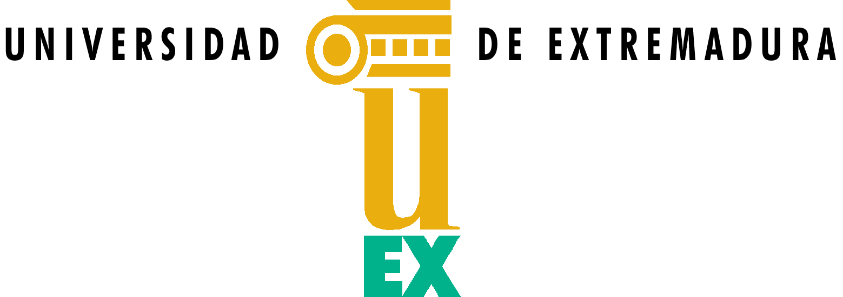
\includegraphics[width=0.8\textwidth]{image.png}} %Para ajustar la portada a una sola página se puede reducir el tamaño del logo
\vspace{3.0cm}}


\author{\IEEEauthorblockN{Álvaro Gonzalez Antequera}
\IEEEauthorblockA{\textit{Robotics Group 5} \\
Cáceres, Spain \\
agonzaleyn@alumnos.unex.es}
\and
\IEEEauthorblockN{Aarón Ventura Matito}
\IEEEauthorblockA{\textit{Robotics Group 5} \\
Cáceres, Spain \\
aaventura@alumnos.unex.es}

\vspace{20.0 cm}
}


\maketitle

\subsection{INDEX}
\begin{itemize}
    \item INTRODUCTION
    \begin{itemize}
        \item Autonomics Robots
        \end{itemize}
    \item ACTIVITY 1
        \begin{itemize}
        \item Description of the problem 
        \item Proposed solution
        \end{itemize}
\end{itemize}



\section{Introduction}




\subsection{Autonomics robots}

Software for autonomous robotic systems typically operates within an embedded, concurrent, real-time, and distributed environment, handling a substantial amount of data. It is imperative to ensure system attributes such as safety, reliability, and fault tolerance. Presently, most of the research and development in robotics still relies on individually crafted software architectures created from scratch for each project. Numerous valuable robotic applications are self-contained systems specifically designed to address particular problem categories.

Consequently, there exists a substantial reservoir of software applications that encompass the complete range of robot functions, algorithms, and control paradigms within robotics research facilities. Regrettably, these applications are often non-reusable in slightly different use cases due to their strong dependencies on particular robot hardware, processing platforms, and communication infrastructures. Additionally, these applications tend to have embedded assumptions and constraints related to tasks and operational environments that are challenging to modify in the software's implementation.

Our primary framework for this project revolves around Webots. This is employed for rapid algorithm development, factory automation simulations, swift prototyping and validation, educational purposes in robotics, remote monitoring, safety verification, acting as a digital twin, and much more. For a comprehensive overview of its features, you can find more information in following link: https://cyberbotics.com .


\section{ACTIVITY 1 }


\subsection{Description of the problem}\label{AA}
The execution of this practice is carried out in the Webots simulator, which we will use in all the subject's exercises, along with other components. In this section of the practice "Introduction to component-oriented programming and robot control," we are tasked with achieving automatic movement for our robot, which needs to navigate among obstacles while avoiding collisions. To accomplish this, it is necessary to establish the connection between perception and action to generate a specific behavior. The robot must go through four different states.

\subsection{Proposed solutions}
The execution of this practice is carried out in the Webots simulator, which we will use in conjunction with other components. In this practice, we are tasked with achieving automatic movement for our robot, which needs to navigate among obstacles while avoiding collisions. To accomplish this, it is necessary to establish the connection between perception and action to generate a specific behavior. The robot must go through four different states (which we will see below) in both an automated and random manner to achieve the most efficient movement on the surface where it is located.

The different states that the robot can transition through are as follows:

\begin{itemize}
    \item \textbf{STRAIGHT-LINE:} This state directs the robot to move in a straight line, serving as the base state for robot movement.
    \item \textbf{FOLLOW-WALL:} In this state, the robot primarily moves parallel to a wall when it approaches one.
    \item \textbf{SPIRAL:} The robot follows a specific spiral pattern in this state until it approaches a wall.
    \item \textbf{TURN:} This state instructs the robot to rotate around itself.
    \item \textbf{MIDDLE:} Regardless of its initial position, the robot moves toward the center of the surface in this state.
\end{itemize}
     

\subsection{Results obtained}
Once the proposed solution was implemented and tested, we assessed the robot's performance within the Webots environment. The different results obtained in all the tests we conducted were relatively similar. However, depending on various factors, the outcome varied, either improving or deteriorating. The factors that influenced the effectiveness of the robot's movement are as follows:

\begin{description}
    \item[-Degree of randomness]
    \item[-Obstacles]
\end{description}   
\vspace{1.0 cm}

\subsubsection{Degree of randomness}
In this practice, the robot has been tested in two ways in terms of randomness.

The following diagrams show the state options that the robot can choose from depending on the degree of randomness:

\begin{figure}
  \centering
  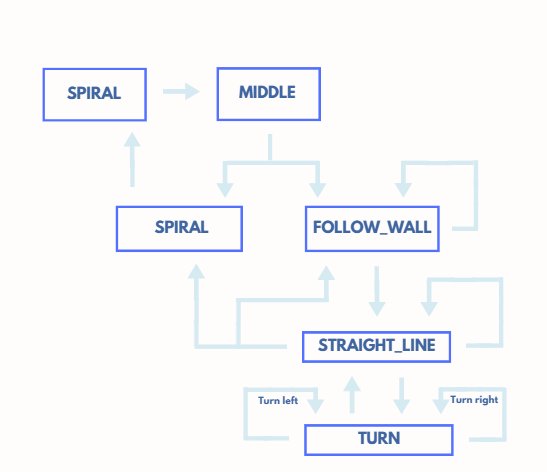
\includegraphics[width=0.4\textwidth]{DiagramaCon.png}
  \caption{with randomness}
  \label{fig:with randomness}

  \vspace{1.0 cm}
  
  \centering
  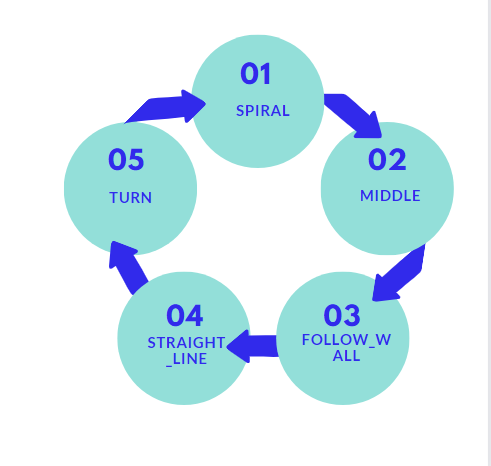
\includegraphics[width=0.4\textwidth]{DiagramaSin.png}
  \caption{without randomness}
  \label{fig:without randomness}

  
\end{figure}

  \vspace{10.0 cm}

-The first way has been through state changes, excluding the introduction of randomness. In other words, the Trial and Error principle has been used to determine, with the implemented code, the best way the robot could move on the surface. In these tests, no Obstacle Objects have been introduced. As you can see, without the Random characteristic, the robot follows the same procedure in all three tests, meaning that the sequence of States is the same, and therefore the next:

    SPIRAL - MIDDLE - FOLLOWWALL - TURN - STRAIGHTLINE

\begin{figure}
  \centering
  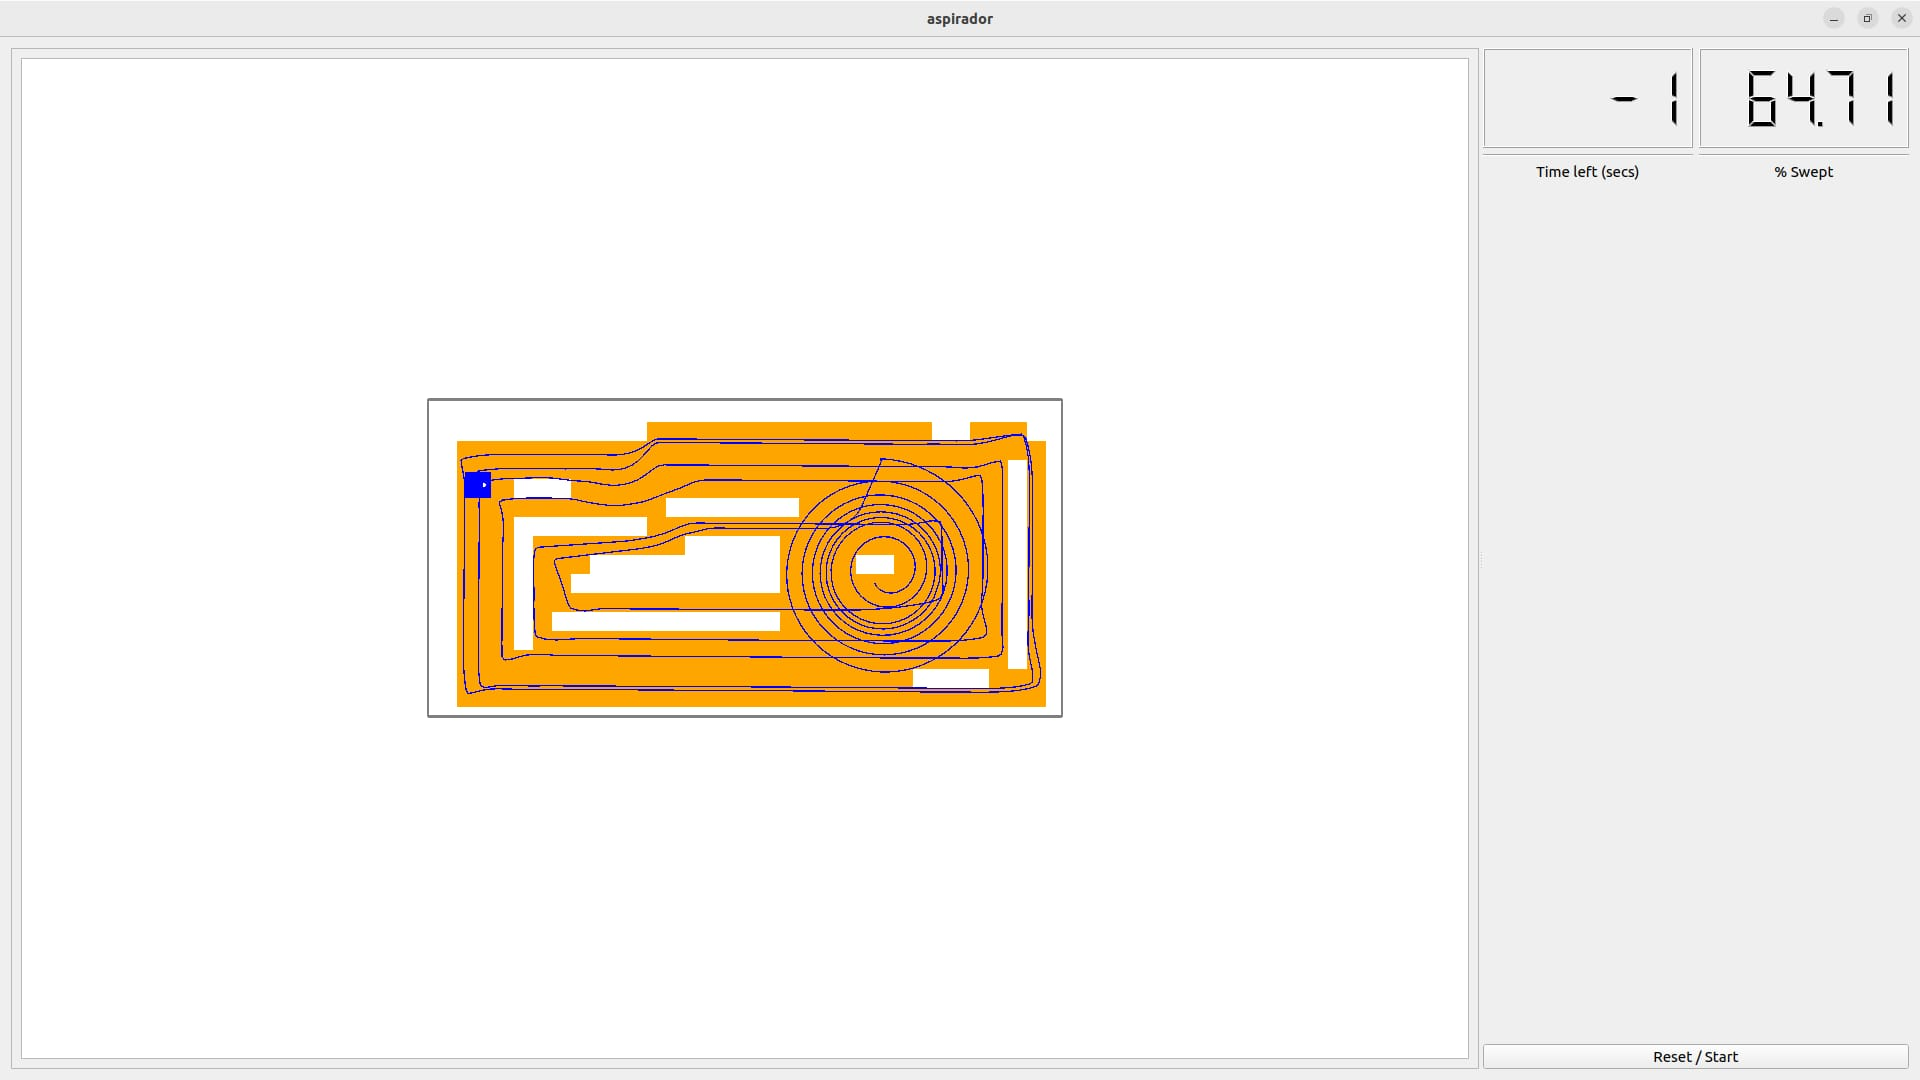
\includegraphics[width=0.4\textwidth]{test1sin.jpg}
  \caption{Test 1}
  \label{fig:Test 1 sin aleatoriedad}

  \vspace{1.0 cm}
  
  \centering
  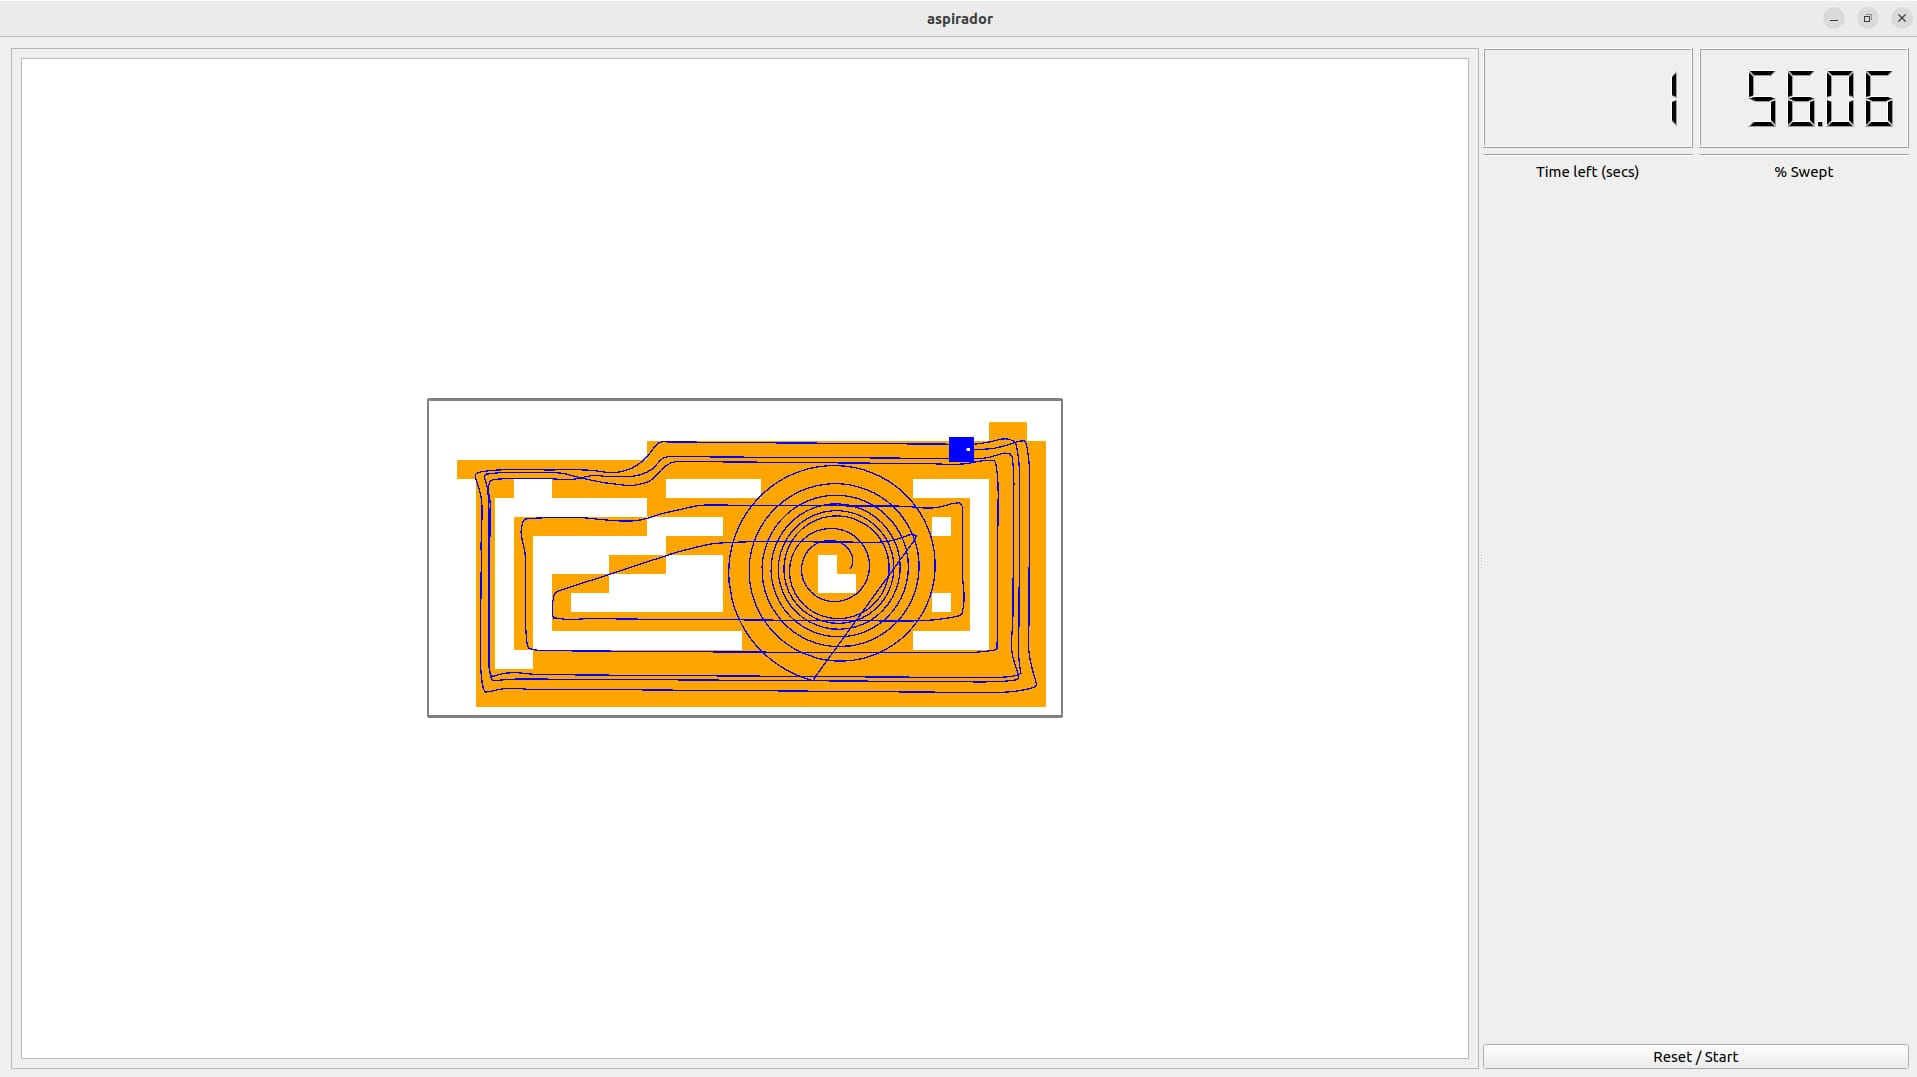
\includegraphics[width=0.4\textwidth]{test2sin.jpg}
  \caption{test 2}
  \label{fig:Test 2 sin aleatoriedad}

  \vspace{1.0 cm}

  \centering
  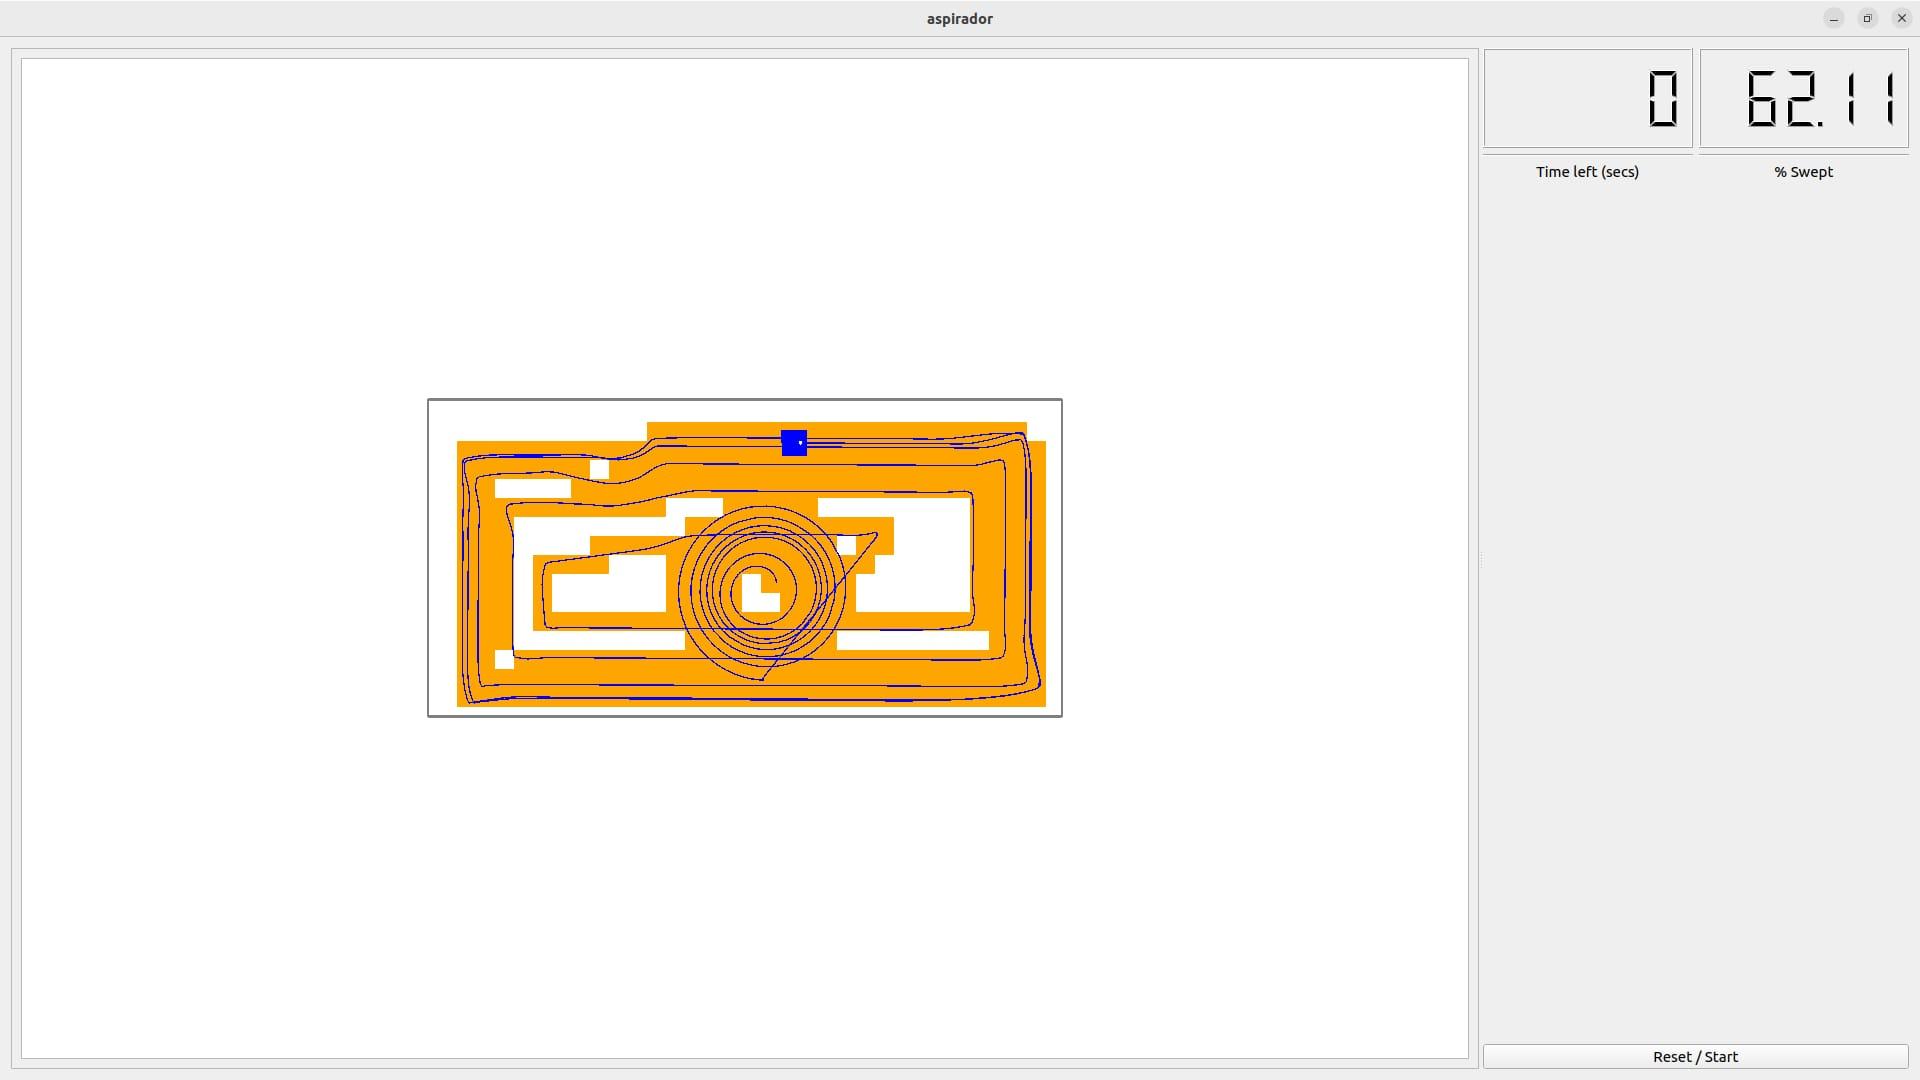
\includegraphics[width=0.4\textwidth]{test3sin.jpg}
  \caption{test 3}
  \label{fig:Test 3 sin aleatoriedad}
  
\end{figure}

\vspace{10.0 cm}


- The second way is by adding Randomness. In this case, randomness is implemented in the robot's state changes. Depending on the state it is in at any given moment, the robot can switch from one state to another. For this approach, three tests have also been conducted.

\vspace{3.0 cm}

\begin{figure}
  \centering
  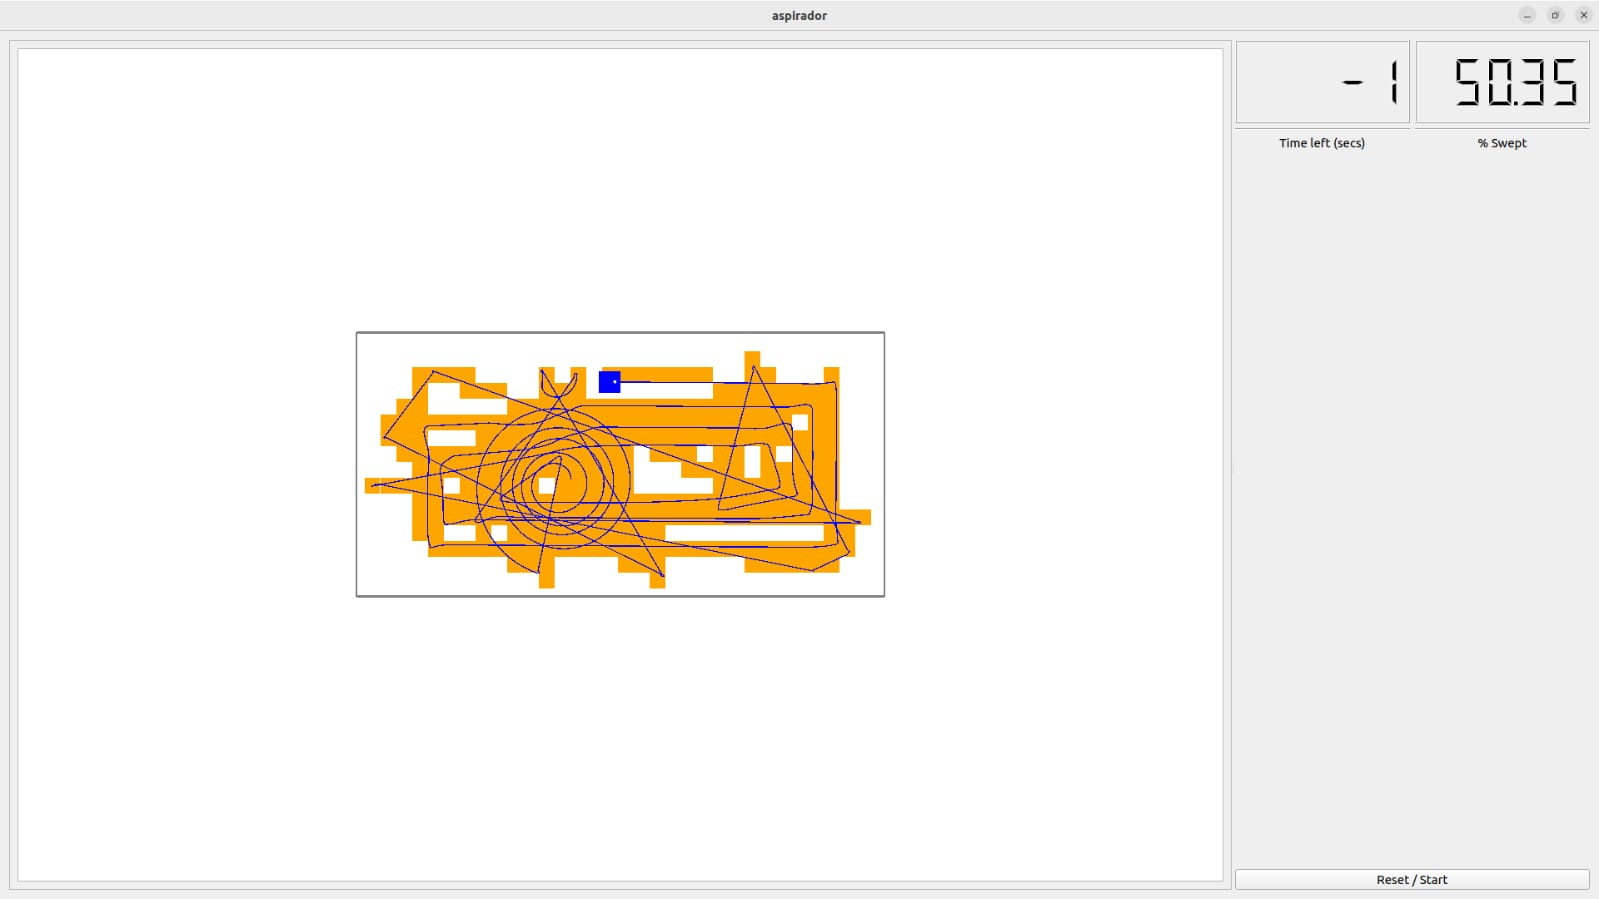
\includegraphics[width=0.4\textwidth]{test1con.jpg}
  \caption{Test 1 random}
  \label{fig:Test 1 con aleatoriedad}

  \vspace{1.0 cm}
  
  \centering
  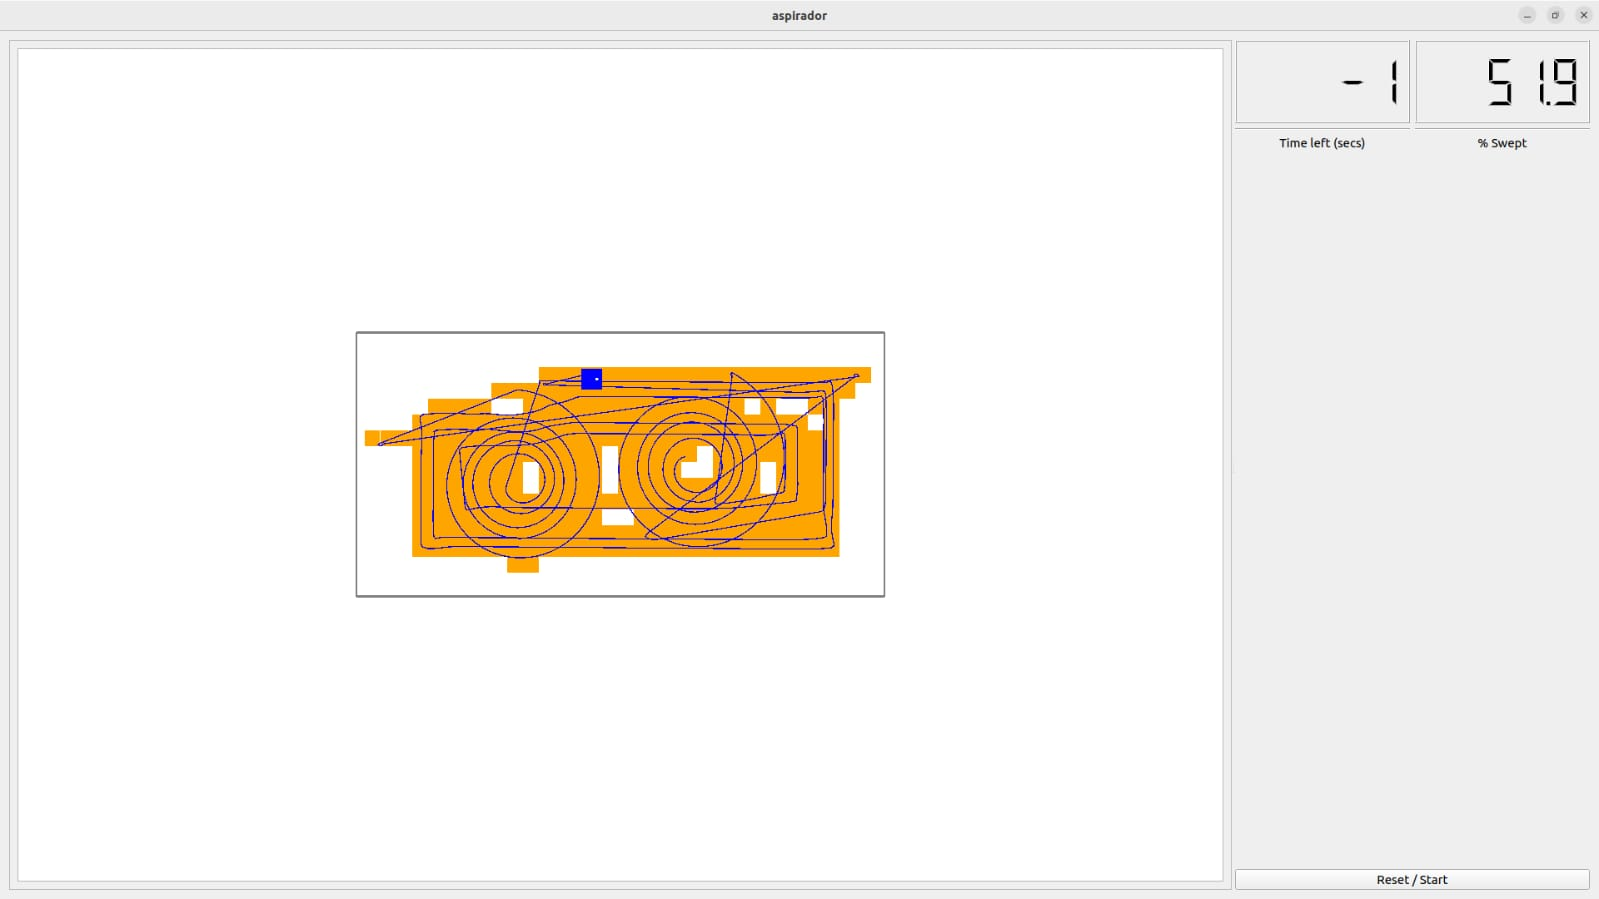
\includegraphics[width=0.4\textwidth]{test2con.jpg}
  \caption{Test 2 random}
  \label{fig:Test 2 con aleatoriedad}

  \vspace{1.0 cm}

  \centering
  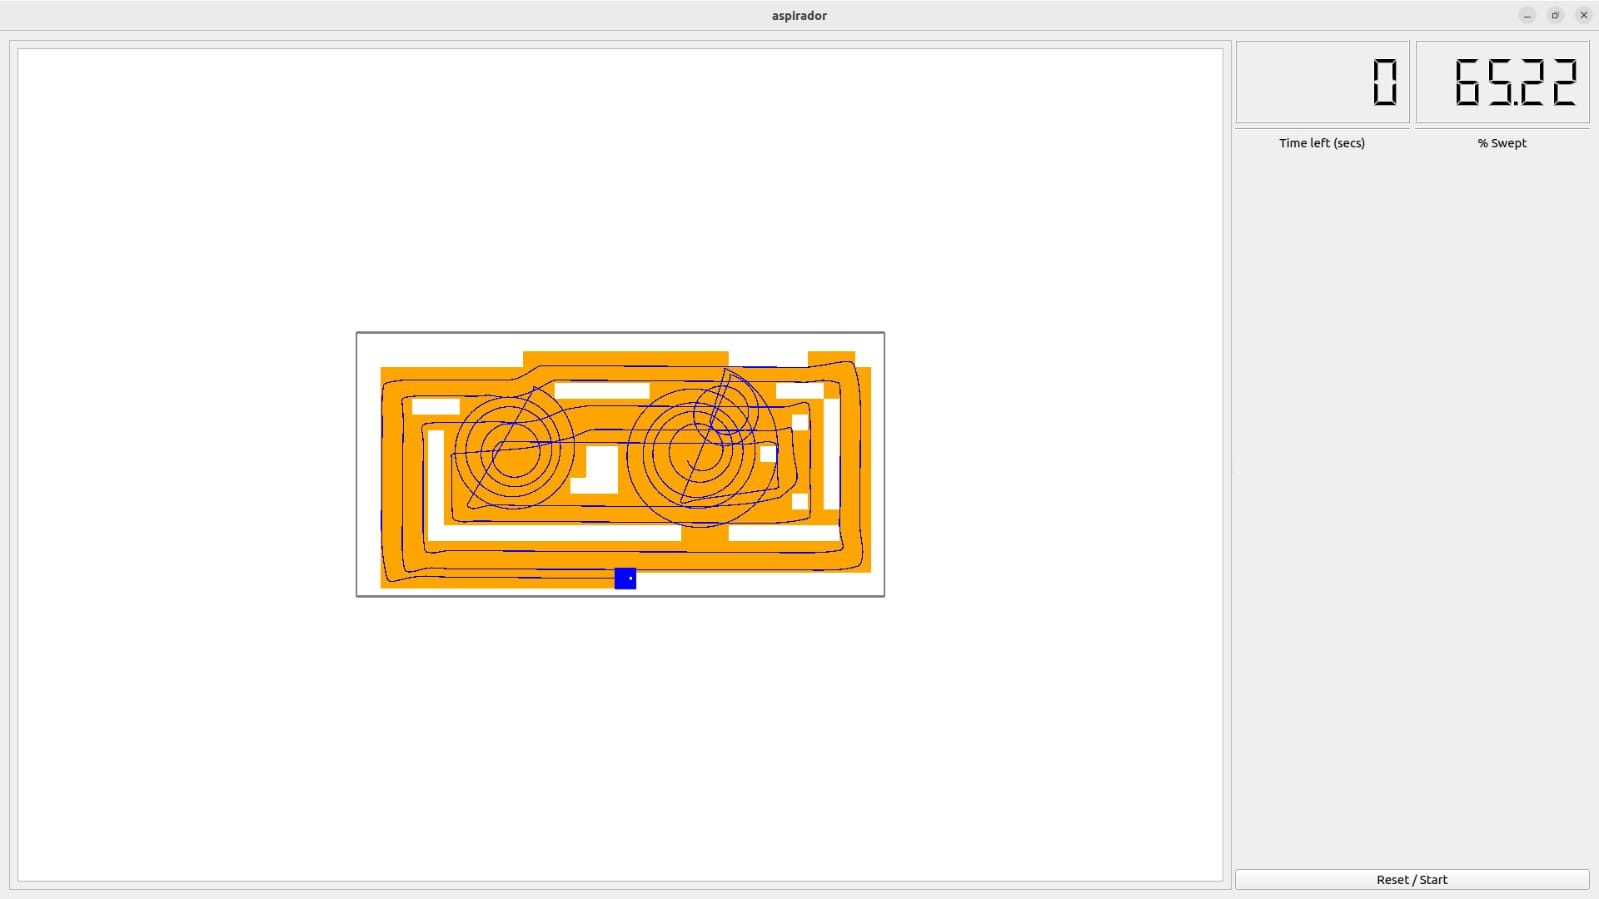
\includegraphics[width=0.4\textwidth]{test3con.jpg}
  \caption{Test 3 random}
  \label{fig:Test 3 con aleatoriedad}
  
\end{figure}

\vspace{3.0 cm}


- Finally, with the Randomness feature activated, objects were introduced into the robot's test environment. These objects were boxes of the same size, placed in different locations within the environment to observe the behavior of the robot's Randomness in an environment with obstacles.

\begin{figure}[!htb]
  \centering
  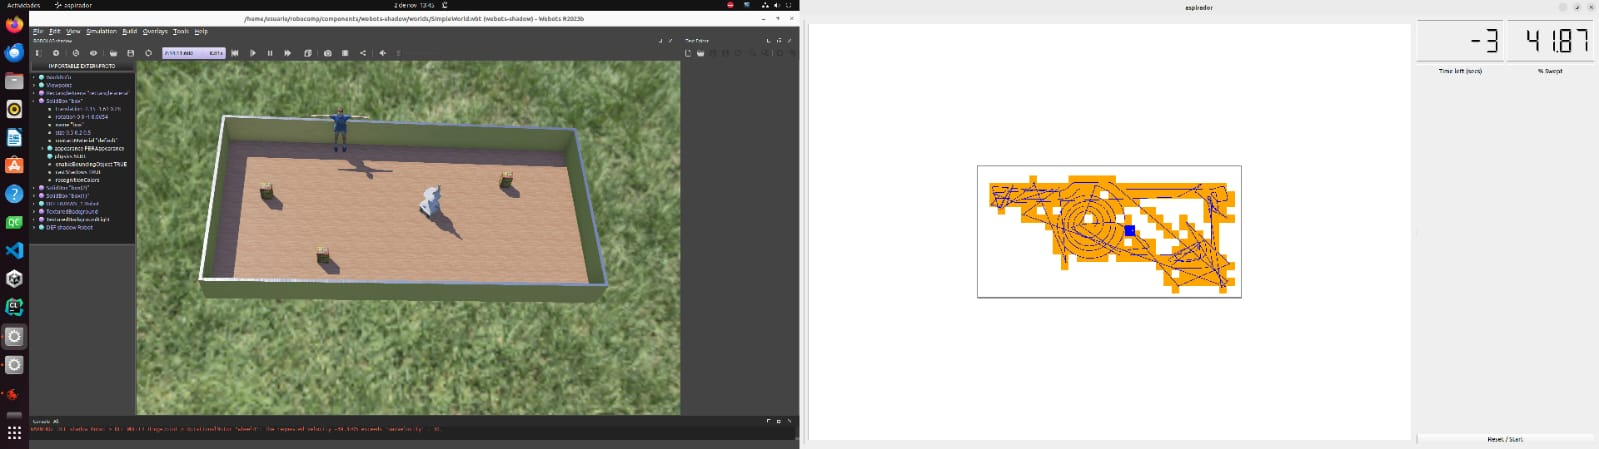
\includegraphics[width=0.4\textwidth]{objetos.jpg}
  \caption{Test with obstacles}
  \label{fig:Test con aleatoriedad y cajas}
\end{figure}

Github link -- https://github.com/aaventuramatito/grupo5-robotica2023

\end{document}



















